\documentclass{beamer}
\usetheme{afm}

\title{Bootrstrap Technique}
\author{\href{mailto:matteo.sani@unisi.it}{Matteo Sani}}

\begin{document}
\begin{frame}[plain]
  \maketitle
\end{frame}

\begin{frame}{Overnight Index Swap}
\begin{itemize}
\item Interest rate swaps (IRS) are usually used to mitigate the risks of fluctuations of interest rates, or to benefit from lower rates. 
\item An Overnight Index Swap (OIS) is a particular kind of IRS which pays a floating coupon, determined a pre-determined index of a daily overnight reference rate (e.g €STR), against a fixed coupon.  
\item An OIS is defined by:
\begin{itemize}
  \item a notional amount $N$;
  \item a starting date $d_0$;
  \item a sequence of payment dates $d_1,...,d_n$;
  \item a fixed rate $K$.
\end{itemize}
\item For simplicity in the following we assume the fixed and floating legs to have the same notional and payment dates, although this is not necessarily always the case in practice.
\end{itemize}
\end{frame}

\begin{frame}{OIS Valuation}
\begin{itemize}
\item To compute the NPV of such products it is necessary to sum the discounted values of each leg cash flows (full derivation in the notes)
\begin{tabular}{|c|c|}
\hline
 Floating Leg & Fixed Leg \\
\hline
$\mathrm{NPV}_{\mathrm{float}} = N \cdot [D_{\mathrm{OIS}}(d_0) - D_{\mathrm{OIS}}(d_n)]$ & $\mathrm{NPV}_{\mathrm{fixed}} = N\cdot K\cdot \sum_{i=1}^{n}D_{\mathrm{OIS}}(d_{i})\frac{d_i - d_{i-1}}{360}$ \\
\hline
\end{tabular}
\\\vspace{0.05cm}
where $D_{\mathrm{OIS}}(d)$ is the discount factors implied by OIS prices (\textbf{we will see how to derive it}).
\item We will always look at these products from the point of view of the \emph{receiver of the floating leg}
\begin{equation}
\mathrm{NPV}_{\mathrm{OIS}} = \mathrm{NPV}_{\mathrm{float}} - \mathrm{NPV}_{\mathrm{fixed}}
\end{equation}
\item The $\frac{1}{360}$ fraction appears because €STR rates are quoted using the ACT/360 day-count convention:
\begin{itemize} 
  \item other currencies might have different conventions;  
  \item in addition we are making the simplifying assumption of ignoring weekends and holidays: each overnight rate is valid for only one day.
  \end{itemize}
\end{itemize}
\end{frame}

%\begin{frame}{OvernightIndexSwap Class}
%\begin{itemize}
%\item Let's write a class to represent OIS and compute its value given a specific discount curve
%\begin{itemize}
%    \item attributes: start_date, nominal, fixed leg rate and payment dates;
%    \item methods: two to compute NPVs of floating and fixed legs respectively and one to compute the swap value. 
%    \end{itemize}
% \item In order to avoid future bugs and to provide users with the correct information to use a class it is always a good practice to document your code.
% \item Documentation can be written inline beside the class code using multiline strings ($\texttt{"""}$) below each method to describe the purpose and the needed parameters.
% 
%# define OIS class
%from finmarkets import generate_dates
%
%class OvernightIndexSwap:
%  """
%  Class to manage Overnight Index Swap contracts
%  Parameters:
%  nominal: the nominal of the contract
%  start_date: the initial date of the contract
%  maturity_months: the maturity to be expressed in months 
%  fixed_rate: rate of the "fixed leg"
%  """
%  def __init__(self, nominal, start_date, maturity_months, fixed_rate):
%      self.start_date = start_date
%      self.nominal = nominal
%      self.fixed_rate = fixed_rate
%      self.payment_dates = generate_dates(start_date, maturity_months)
%      
%  def npv_floating(self, dc):
%    """
%    Method to compute the floating leg NPV
%    Parameters:
%    dc: dicscount curve to be used in the calculation
%    """
%    return self.nominal * (dc.df(self.payment_dates[0]) - dc.df(self.payment_dates[-1]))
%  
%  def npv_fixed(self, dc):
%    """
%    Method to compute the fixed leg NPV
%    Parameters:
%    dc: dicscount curve to be used in the calculation
%    """
%    val = 0
%    for i in range(1, len(self.payment_dates)):
%        val += dc.df(self.payment_dates[i]) * \
%                (self.payment_dates[i] - self.payment_dates[i-1]).days/360 
%    return self.nominal*self.fixed_rate*val
%  
%  def npv(self, dc):
%    """
%    Method to compute the contract NPV seen from the point of view of the 
%    receiver of the floating leg.
%    Parameters:
%    dc: dicscount curve to be used in the calculation
%    """
%    return self.npv_floating(dc) - self.npv_fixed(dc)
%        
% #### Example
% 
% * Let's test the class with this [discount curve](https://github.com/matteosan1/finance_course/raw/develop/libro/input_files/discount_factors_2022-10-05.xlsx).
% 
%# test the class
%import pandas as pd
%from datetime import date
%from finmarkets import DiscountCurve
%from dateutil.relativedelta import relativedelta
%
%start_date = date(2020, 10, 21)
%ois = OvernightIndexSwap(1e6,
%                         start_date, 
%                         36,
%                         0.025)
%
%df = pd.read_excel("https://github.com/matteosan1/finance_course/raw/develop/libro/input_files/discount_factors_2022-10-05.xlsx")
%pillars = [start_date + relativedelta(months=i) for i in df['months']]
%dfs = df['dfs']
%
%curve = DiscountCurve(pillars, dfs)
%
%print ("OIS NPV: {:.2f}".format(ois.npv(curve)))
%
%OIS NPV: -2096.44

\begin{frame}{Discount Factor Determination (Bootstrap)}
\begin{itemize}
\item Our ultimate goal is to take a series of Overnight Index Swap quotations, and determine the discount factors implied by their prices. 
\item The employed technique is called \emph{bootstrap}: this is the ABC of financial mathematics, since you always need a discount curve to price a contract.
\item We concentrate on €STR swaps in order to build an EUR discount curve.
\item The asumption underlying bootstrap is that market quotes represent the \emph{fair} prices of the OIS:
\begin{itemize}
  \item by fair price we mean an estimate of what a willing buyer would pay a willing seller for a given asset, assuming both have a reasonable knowledge of the asset's worthness;
  \item by defintion market quotes make the swap NPVs null.
  \end{itemize}
  \end{itemize}
\end{frame}  
  
\begin{frame}{The Algorithm}
\begin{itemize} 
\item In finance, \emph{bootstrap} is a method for constructing a yield curve from the prices of a set of coupon-bearing products (e.g. bonds and swaps) using only few selected products, it is possible to derive rates for all possible maturities.
\item The term structure of spot rates is obtained from the yields by \emph{forward substitution}, in other words by solving for them recursively. 
\end{itemize}
\end{frame} 

\begin{frame}[fragile]{Example}
\begin{itemize}
\item Consider five bonds (yearly fixed coupon of 4\%, 5\%, 6\%, 7\% and 8\% respectively) with maturities ranging from 1 to 5 years, each having a value of €100 and \emph{traded at par} (traded at its face value). 
\item To determine the yield curve proceed as follows:
\begin{enumerate}
   \item at the end of first year the discounted cash flow of the first bond is €104 (principal + coupon) times the discount factor, so the implied 1 year rate can be found by solving
   \begin{equation*}
 100 = \cfrac{104}{(1 + r_{1y})}\implies r_{1y} =  104/100 - 1 = 4\%
 \end{equation*}
 \item at the end of second year the sum of the cash flows of the second bond can be compared to its trading price to compute the 2-year spot rate $r_{2y}$ (using the previously derived value of $r_{1y}$)
    \begin{equation*}
    \begin{gathered}
 100 = \cfrac{5}{(1 + r_{1y})} + \cfrac{105}{(1 + r_{2y})^{2}} \\
 100 = 5 / (1 + 0.04) + 105 / (1 + r_{2y})^{2}\qquad\Rightarrow\qquad r_{2y}^2  + 2 r_{2y}  - 0.103030 = 0
 \end{gathered}
 \end{equation*}
 \end{enumerate}
 \end{itemize}
\end{frame}
 
\begin{frame}[fragile]{Example}
\begin{itemize}
 This second order equation can be solved either by hand or with \texttt{numpy.roots}.
 \begin{equation*}
    r_{2y} = - 1 \pm \sqrt{1 + 0.103030} = \begin{cases}-2.05023 \\ 0.0502\end{cases}
    \end{equation*}
    
 \begin{ipython}
import numpy as np
np.roots([1, 2, -0.103030])
 \end{ipython}
 \begin{ioutput}
 array([-2.05025235,  0.05025235])
\end{ioutput}
\item From the third year on we get equation of third order (or more) which are not easily analitically solvable (fifth year):
 \begin{equation*}
 100 = \cfrac{8} {(1 + r_{1y})} + \cfrac{8} {(1 + r_{2y})^{2}}+ \cfrac{8} {(1 + r_{3y})^{3}} + \cfrac{8} {(1 + r_{4y})^{4}} + \cfrac{108} {(1 + r_{5y})^{5}}
 \end{equation*}
\end{itemize}
\end{frame}  
 
 \begin{frame}[fragile]{Example}
 \begin{itemize}
 \item Assuming we have already determined the previous rates:
 \begin{tabular}{|c|c|c|c|}
 \hline
  years & coupon rate & bond price & rate \\
 \hline
 1 & 1\% & 100 & 4.00\% \\
 \hline
 2 & 2\% & 100 & 5.02\% \\
 \hline
 3 & 3\% & 100 & 6.08\% \\
 \hline
 4 & 4\% & 100 & 7.19\% \\
 \hline
 5 & 5\% & 100 & ???? \\
 \hline
 \end{tabular}
 
 \item Solving the previous equation means to find its zeros: the values of $\hat{x}$ for which $f(\hat{x})=0$.
 \item There are various methods to solve this problem (which is also called root-finding), the simplest being the \emph{bisection method}.
% ![](https://drive.google.com/uc?id=1Zt18h9fRo65Er5V9iJBdOpX4trcytLSW)
 \end{itemize}
 \end{frame} 
 
\begin{frame}[fragile]{Example}
\begin{itemize}
 \item In \emph{python} this algorithm is implemented in \texttt{scipy.optimize.bisect}.
 
\begin{ipython}
import numpy as np
from scipy.optimize import bisect
 
def f(y):
    return 8/(1+0.04) + 8/np.power((1+0.0502), 2) + 8/np.power((1+0.0608), 3) + 8/np.power((1+0.0719), 4) + 108/np.power((1+y), 5) - 100
 
print (f"{bisect(f, 0, 1):.4f}")
\end{ipython}
\begin{ioutput} 
 0.08359
\end{ioutput} 
\item An interesting alternative is the \emph{Brent method} available in \texttt{scipy.optimize.brentq}.

\begin{ipython}
from scipy.optimize import brentq
 
print (f"{brentq(f, 0, 1):.4f}")
\end{ipython}
\begin{ioutput} 
 0.08359
\end{ioutput} 
 \end{itemize}
 \end{frame} 
 
\begin{frame}[fragile]{Example}
\begin{itemize}
\item The very same mechanism can be generalized to more maturities to get a more detailed yield curve: 
 
\begin{equation*}
 \begin{cases}
 f_1(r_1, p_1) = 0 \\
 f_2(r_1, r_2, p_2) = 0 \\
 f_3(r_1, r_2, r_3, p_3) = 0 \\
 f_4(r_1, r_2, r_3, r_4, p_4) = 0 \\
 \cdots
 \end{cases}
 \end{equation*}
where $r_i$ are the unknown spot rates and $p_i$ the market quotes of the considered products. 
 
 \item The iterative procedure we have applied before exploits the first equation to find $r_1 = f_1^{-1}(p_1)$, the second to find $r_2 = f_2^{-1}(r_1, p_2)$ and so on...
\end{itemize}
\end{frame} 
 
\begin{frame}{Minimization Algorithm}
\begin{itemize} 
\begin{ * Let's see how a minimization algorithm works looking at a practical example.
 * Find the dimensions that will minimize the costs to manufacture a cylindrical can of volume $330~\mathrm{cm}^3\;(33~\mathrm{cl})$:
   * **cheaper can -> less aluminum -> smaller surface given the volume**
 
 <center>
 
 ![](https://drive.google.com/uc?id=1LQaX8j10nq1KgRu4RdR4Ade96fsMNxa6)
 
 </center>
 
 $$ S(r, h) = 2\pi rh + 2\cdot(\pi r^2) $$
 
 * The volume is fixed to $330~\mathrm{cm}^3$ so we can remove $h$ from the previous equation:
 
 $$ V = \pi r^2 h = 330\quad\implies h = \cfrac{330}{\pi r^2} $$
 
 * The surface function to be minimized is:
 
 $$ S(r) = 2\pi rh + 2\cdot(\pi r^2) = \cfrac{2\cdot 330}{r} + 2\cdot(\pi r^2)$$
 
 
   1. define an *objective function* i.e. the function that is actually minimized to reach our goal (in this example the can area function);
    2. set the initial value of the unknown parameters and their range of variability; we are going to start with $r=1~\mathrm{cm}$ and let it varies between $1~\textrm{mm}$ and $1~\textrm{m}$;
   3. Finally run the algorithm (it is defined in `scipy.optimize.minimize`):
     * compute the objective function value;
     * move the parameter values ($r$ in our example) to find a smaller value of the objective function (e.g. following the derivative direction w.r.t. each parameter); in case constraints are defined, they will be considered when the parameter values are varied;
     * repeat until further variations of the values won’t change significantly the objective function (i.e. we have found a minimum of the function so the minimization process is completed !).
     
 ## Back to OIS Bootstrap
 
 * In the latter formulation we gave bootstrap requires to minimize simultaneously the NPV's of a set of OIS;
 
 $$\begin{equation}
 \mathrm{Objective Function} =	f_1^2(\hat{r}_1,p_1) + f_2^2(\hat{r}_1, \hat{r}_2,p_2) + \ldots =\sum_{i=1}^{n}\mathrm{NPV}^\mathrm{OIS}_i(\mathcal{C})^2
 \end{equation}$$
 
 * The only unknown parameter of each NPV is the discount curve $\mathcal{C}$ (i.e. **the algorithm will adjust the unknown discount factors of $\mathcal{C}$ to reach the minimum**).
   * In the previous example there was a single parameter involved in the minimization i.e. the can radius.
   * A discount curve is characterized by pillar dates ($\mathbf{d}$) and discount factors ($\mathbf{x}$):
       * we haven't yet identified a constraint on how many points the curve needs to be made of (*too many or too few points may prevent us from finding the solution*).
   * **It makes sense to choose the number of parameters (degrees of freedom) to match the number of market quotes** (set the pillar dates equal to the set of the swap expiry dates).
 
 $$\begin{equation}
  \mathrm{min}_{\mathbf{x}} \left\{\sum_{i=1}^{N}\mathrm{NPV}^\mathrm{OIS}_i( \mathcal{C}(\mathbf{x}))^2\right\}
 \end{equation}$$
 
 * First create the swaps according to the available market quotes:
 
 The file can be downloaded from here: [ois_2022_09_30.xlsx](https://github.com/matteosan1/finance_course/raw/develop/libro/input_files/ois_2022_09_30.xlsx)
 
      
 
    
    



\begin{frame}{The Course}
  \begin{itemize}
  \item Official WebSite: \href{https://sites.google.com/view/finmark2023}{https://sites.google.com/view/finmark2023}
  \item Facebook Group: \href{https://www.facebook.com/groups/628149578705431}{https://www.facebook.com/groups/628149578705431}
  \item \textbf{The course consists of about 10 lessons (Wednesday 18.00 - 19.30) in Aula Informatica 2.}
  \item The goal is to \emph{provide you with the basic numerical tools developed with \texttt{python} to solve real world financial problems.}
  \end{itemize}
\end{frame}

\begin{frame}{Topics}
  \begin{columns}
    \column{0.5\linewidth}
    \begin{block}{Mathematical Techniques}
      \begin{itemize}
      \item interpolation;
      \item bootstrapping;
      \item Monte Carlo simulation;
      \item copulas;
      \item numerical optimization.
      \end{itemize}
    \end{block}
    \column{0.5\linewidth}
    \begin{block}{Financial Topics}
      \begin{itemize}
      \item bonds;
      \item pricing of IR and Credit derivatives;
      \item Value at Risk, credit risk;
      \item Credit Value Adjustment;
      \item portfolio optimization.
      \end{itemize}
    \end{block}
  \end{columns}
  \begin{block}{Machine Learning (ML)}
    \begin{itemize}
    \item basic deep learning theory;
    \item ML financial application (Neural Networks, Convolutional Networks..).
    \end{itemize}
  \end{block}
\end{frame}

\begin{frame}{Topics}
  \begin{itemize}
    \item Lecture notes are available on the website with additional material available there exercises (with solutions). 
    \item You are encouraged to do the exercises and send me by email your homework (I will correct and give you some feedback on what you have done !).
    \item \textbf{For every doubt or question do not hesitate to contact me, I am always available at the above email addresses and usually quite responsive.}
  \end{itemize}
\end{frame}

\begin{frame}{Why \texttt{python} ?}
  \begin{itemize}
  \item \texttt{python} is widely used \textbf{even if it is slower than other languages} because:
    \begin{itemize}
    \item it is a productive, very concise and expressive language and requires little time, effort, and lines of code to perform the same operations than with other languages;
    \item it has a rich set of libraries and frameworks;
    \item it is maintained by a large community of users.
    \end{itemize}

    \item \textbf{But unfortunately not all that glitters is gold !}

    \item \texttt{python} is an interpreted language: it takes a sequence of instructions, reads and executes it.
  \end{itemize}
  
  \begin{columns}
    \column{0.35\linewidth}
    This is different from other programming languages like \texttt{C} or \texttt{C++} which compile code into a language that computers can understand directly (\emph{machine language}).
    \column{0.65\linewidth}
    \begin{figure}[h]
      \begin{center}
        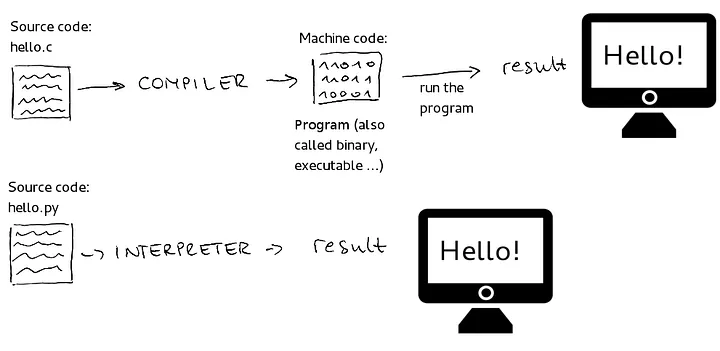
\includegraphics[width=0.8\linewidth]{compiled_vs_interpreted}
      \end{center}
    \end{figure}
  \end{columns}
\end{frame}

\begin{frame}{Compiled vs Interpreted}
  \begin{itemize}
  \item As a result, \texttt{python} is essentially an interactive programming language.
  \item You can program and see the results almost at the same time. 
  \item \emph{Very nice} when developing a new project since \emph{compilation time} can be quite long (just to give an idea the compilation of our \texttt{C++} financial code takes about one hour). 
  \item However there are \textbf{drawbacks} in term of performance, the translation to machine language has to be done in real-time resulting in slower execution times.
  \end{itemize}
\end{frame}

\begin{frame}{\texttt{Python} Language Recap}
  \begin{itemize}
    \item Most of you should be already accustomed to \texttt{python}.
    \item Anyway the first few Chapters of the \href{https://drive.google.com/file/d/1fuVzryJwMCilgynwS7VbWKAmKQBojMQs/view?usp=sharing}{lecture notes} cover in some detail its main features.
    \item Otherwise you can take a look at one of the thousands \texttt{python} tutorials available on the web.
    \item Just look at some more advanced aspects here.
  \end{itemize}
\end{frame}

\begin{frame}[fragile]{Modules}
  \begin{itemize}
  \item Frequently used functions can be written in a \emph{module} and \emph{import} it, instead of copying their definitions into different programs many times.
  \item In essence modules refer to a file containing \texttt{python} code and used to break down large programs into small manageable and organized files. 
  \item There are thousands of modules available for \texttt{python} and you can also write your own and distribute it to the community.
  \item \textbf{The modules we are going to use most are: \texttt{pandas}, \texttt{datetime}, \texttt{matplotlib}, \texttt{scipy}, \texttt{numpy}, \texttt{math}}
  \item  Lecture notes contain a dedicated Chapter to the first three of them.
  \end{itemize}
\end{frame}

\begin{frame}[fragile]{Modules}
\begin{ipython}
import math
help(math)
\end{ipython}
\begin{ioutput}
Help on built-in module math:

NAME
    math

DESCRIPTION
    This module provides access to the mathematical functions
    defined by the C standard.

FUNCTIONS
    acos(x, /)
        Return the arc cosine (measured in radians) of x.
\end{ioutput}
\begin{ipython}
dir(math)
\end{ipython}
\begin{ioutput}
['__doc__', '__loader__', '__name__', '__package__', '__spec__', 'acos',
 'acosh', 'asin', 'asinh', 'atan', 'atan2', 'atanh', ...
\end{ioutput}    
\end{frame}

\begin{frame}[fragile]{Using a Module}
  There are several ways to use a module
  \begin{ipython}
# import the submodule pyplot and assign an alias to shorten the name    
import matplotlib.pyplot as plt
import math

# functions inside the module can be accessed as alias.function
plt.show()
math.log(10)

# to avoid prepending the module name in the call
from math import *

log(10)

# finally only specific functions can be imported
from math import log, exp, asin

exp(-4)
asin(0.333)
\end{ipython}
\end{frame}

\begin{frame}[fragile]{\texttt{finmarket} Module}
  \begin{itemize}
  \item Throughout this course we will review the code of a financial module (\texttt{finmarkets}).
  \item We will study and analyze the implementation of most of its functionalities.
  \item Although we are going to write from scratch several parts of the module a working version is available in the official \texttt{python} repository \texttt{pypi}.
  \item In order to make it available for your installation just download it with
\begin{ipython}
pip install --index-url https://test.pypi.org/simple finmarkets
\end{ipython}
  \item Similarly to use it within Google Colab execute a cell with the previous command adding a \texttt{!} in front of the line.
  \end{itemize}
\end{frame}

\begin{frame}[fragile]{\texttt{datetime}}
  \begin{itemize}
  \item We will frequently use \texttt{datetime} module, which is dedicated to date and time.
  \item In addition we rely on \texttt{dateutil.relativedelta} to perform operations on dates (dedicated Sections in the notes).
  \end{itemize}
  \begin{ipython}
from datetime import date
from dateutil.relativedelta import relativedelta
		
d = date.today()
d1 = date(2023, 12, 25)
print (d, d1, (d1 - d).days)
print (d1.strftime('%d/%m/%Y'), d1.weekday())
print (d + relativedelta(days=45))
print (d + relativedelta(months=45))
\end{ipython}
\begin{ioutput}
2022-09-27 2023-12-25 454
25/12/2023 0
2022-11-11
2026-06-27
\end{ioutput}
\end{frame}

\begin{frame}{Payment Dates Generator}
  \begin{itemize}
  \item Since we will need to create many lists of dates (e.g. contract payment dates) let's develop an utility that does that for us.
  \item This is the first example of the utilities implemented in the \texttt{finmarkets} module.
  \item The function we are going to code takes as input
    \begin{itemize}
    \item \emph{starting date} the first date of the list;
    \item \emph{maturity} a string like \texttt{5y} or \texttt{17m} which represents the length of the list (a function in the module take care of converting the string "5y" into the actual number of days in the interval);
    \item \emph{tenor} string like maturity with default value of \texttt{12m}, if the maturity is not a multiple of the tenor the last period will be truncated to the last date.
    \end{itemize}
  \item The function returns a list of dates.
  \end{itemize}		
\end{frame}

\begin{frame}[fragile]{Payment Dates Generator}
  \begin{ipython}
from datetime import date
from dateutil.relativedelta import relativedelta
from finmarkets import maturity_from_str
			
def generate_dates(start_date, maturity, tenor="1y"):
    maturity_months = int(round(maturity_from_str(maturity), 0))
    tenor_months = int(round(maturity_from_str(tenor), 0))
    dates = []
    for d in range(0, maturity_months, tenor_months):
        dates.append(start_date + relativedelta(months=d))
    dates.append(start_date + relativedelta(months=maturity_months))
    return dates
			
print (generate_dates(date(2023, 8, 28), "25m"))
\end{ipython}
\begin{ioutput}
[datetime.date(2023, 8, 28), datetime.date(2024, 8, 28),
 datetime.date(2025, 8, 28), datetime.date(2025, 9, 28)]
\end{ioutput}
\end{frame}

\begin{frame}{Discount Factor}
  \begin{itemize}
  \item A \emph{discount factor} is the number multiplied by a cash flow value to discount it back to its \emph{present value}.
    %\item The factor increases over time (meaning the value gets smaller) as the effect of compounding the discount rate builds over time.
  \item It is related to the \emph{time value of money} i.e. there is a difference between the "future value" of a payment and the "present value" of the same payment.
  \item Consider a payment $F$ that is to be made $t$ years in the future, we calculate the present value as
    \begin{equation}
      PV = \frac{F}{(1+r)^t};\quad PV=F\exp^{-rt}\textrm{ (continouous compounding)}
    \end{equation}
  \item The discount rate $r$ which is used in financial calculations is usually chosen to be equal to the cost of capital, i.e. risk-free rate.
  \end{itemize}
\end{frame}

\begin{frame}{Discount Curve}
  \begin{itemize}
  \item \emph{Discount factors} are usually presented as curves (\emph{discount curves}) where each point represents the discount relative to a future date.
  \item Discount curves are analogous to \emph{yield curves} given the relationship between discount factor and rate.
    \begin{figure}[h]
      \begin{center}
        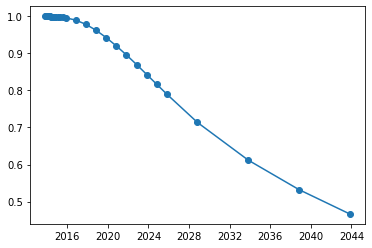
\includegraphics[width=0.55\linewidth]{discount_curve}
      \end{center}
    \end{figure}
  \end{itemize}
\end{frame}

\begin{frame}{Linear Interpolation}
  \begin{itemize}
  \item Since discount factors are available only at discrete times we need a procedure to determine the factors at \emph{every} time; the simplest technique is called \emph{interpolation}.
  \item \emph{Interpolation is a method to "determine" new points within a range of a discrete set of known data points.}
  \item Assume you are traveling by car at \emph{constant speed} (i.e. the traveled distance is $s = v \cdot t$);
    \begin{figure}[h]
      \begin{center}
        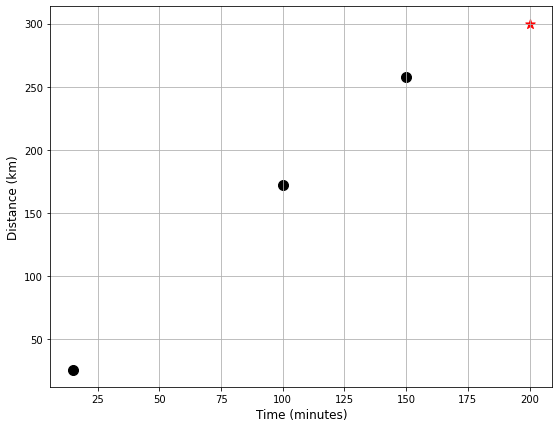
\includegraphics[width=0.45\linewidth]{interp1}
      \end{center}
    \end{figure}
  \end{itemize}
\end{frame}

\begin{frame}[fragile]{Linear Interpolation}
  \begin{itemize}
  \item To find $s(\hat{t})$ at $t_1 \leq \hat{t} \leq t_2$ which is not in our sample we can \emph{linearly interpolate} between two sampled distances $s_1$ and $s_2$ (taken at $t_1$ and $t_2$):
    \begin{itemize}
    \item it works pretty much like a \emph{weighted average} of the two sampled distances (full derivation in the notes);
    \item the closer point has more "influence" than the farther in the result.
    \end{itemize}
  \end{itemize}
  \begin{columns}
    \column{0.5\linewidth}
  \begin{ipython}
from scipy.interpolate import interp1d

t = [15, 100, 150]
s = [25.75, 171.7, 257.7]

interpolator = interp1d(t, s)
print (f"{interpolator(60):.1f}")
\end{ipython}
\begin{ioutput}
103.0
\end{ioutput}
    \column{0.5\linewidth}
    \begin{figure}[h]	
        \begin{center}
        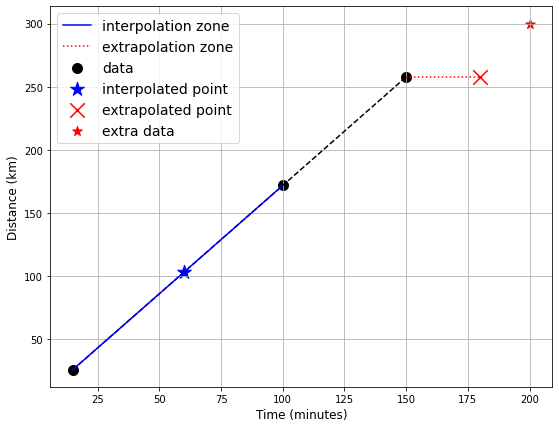
\includegraphics[width=0.85\linewidth]{interp2}
        \end{center}
    \end{figure}
  \end{columns}
\end{frame}

\begin{frame}{Linear Interpolation}
  \begin{block}{Extrapolation}
    If we believe the relation between our variables stays the same (e.g. keep the same constant velocity in our trip), we can also \emph{extrapolate} values \textbf{outside} our initial sample.
    Nevertheless it is quite dangerous to assume a particular trend for our data, so extrapolation should be avoid as much as possible.

    \texttt{interp1d} function by default doesn't allow to extrapolate a result as you can see repeating the previous example replacing 60 with 170 for example.
  \end{block}

  \begin{block}{Always Interpret Critically your Results}
    In this case $t=60$ is almost in the middle of the interval $[t_1, t_2]$, so we expect to get a distance somehow in between $s_1$ and $s_2$, $s(t=60) \approx 100\;\textrm{km}$.
  \end{block}
  \end{frame}

\begin{frame}{Log-linear Interpolation}
  \begin{itemize}
    \item When the function that we want to interpolate is an exponential we can fall back to the previous case by a simple variable transformation. 
      \begin{equation}
        \begin{gathered}
          p = \mathrm{exp}(v \cdot t) \\
          s = \mathrm{log}(p) = \mathrm{log}(\mathrm{exp}(v \cdot t)) = v \cdot t
        \end{gathered}
      \end{equation}

    \item So it is enough to use \texttt{interp1d} with the lists of $t$ and $\log(p)$ and to \emph{exponentiate back at the end} to get the actual value of $p$.
  \end{itemize}
\end{frame}

%\begin{frame}{Limitations of Linear Interpolation}
%  \begin{itemize}
%    \item Interpolation is just an \emph{approximation} and works well when either the function $s$ is linear or we are trying to interpolate between two points that are close enough that $s$ is \emph{almost} linear in that interval;
%    \item intuitively the "curvier" the function the worse the approximation made with simple linear interpolation.
%    \begin{figure}[h]
%      \begin{center}
%        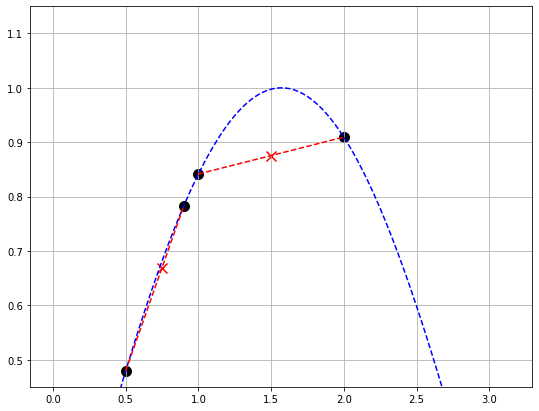
\includegraphics[width=0.55\linewidth]{interp3}
%      \end{center}
%    \end{figure}
%  \end{itemize}
%\end{frame}

\begin{frame}[fragile]{Discount Curve Implementation}
Let's implement a function that given a discount curve return the discount factor at any date.
\begin{ipython}
from datetime import date
from finmarkets import generate_dates
from scipy.interpolate import interp1d
from numpy import log, exp

def df(d, pillars, dfs):
    log_dfs = [log(x) for x in dfs]
    interp = interp1d(pillars, log_dfs)
    return exp(interp(d))
    
pillars = generate_dates(date(2023, 8, 23), '5y')
dfs = [1, 0.98, 0.97, 0.96, 0.95, 0.94]
print (df(date(2024, 3, 15), pillars, dfs))
\end{ipython}
This code won't work ! Indeed \texttt{interp1d} needs two list of \emph{numbers} as $x$ and $y$ but we are passing dates which cannot be interpolated.
\end{frame}

\begin{frame}[fragile]{Second Implementation}
To avoid issues with the dates we need to convert somehow to numbers: the function \texttt{toordinal()} converts indeed a date to the number of days since 0-01-01 (January $1^{st}$, 0).
\begin{ipython}
def df_v2(d, pillars, dfs):
    d = d.toordinal()
    pillars = [d.toordinal() for d in pillars]
    log_dfs = [log(x) for x in dfs]
    interp = interp1d(pillars, log_dfs)
    return exp(interp(d))
    
pillars = generate_dates(date(2023, 8, 23), '5y')
dfs = [1, 0.98, 0.97, 0.96, 0.95, 0.94]
print (df_v2(date(2024, 3, 15), pillars, dfs))
\end{ipython}
\begin{ioutput}
0.9890710382513661
\end{ioutput}
\end{frame}

\begin{frame}{Object Oriented Programming (OOP)}
  \begin{itemize}
  \item Unfortunately having such kind of functions working on "complex" objects like a discount curve is not ideal.
  \item When the number of curves increases it is hard (and error prone) to keep track separately of each list of pillars and factors. It would be better to have a single structure holding the data and the functions acting the that data. 
  \item \emph{Object Oriented Programming is what we need}.
  \item OOP is a programming model where programs are organized around \textbf{objects}, rather than functions and logic.
  \item Every \emph{object} can be thought of as a dataset with unique attributes and a "behavior".
  \item Examples:
    \begin{itemize}
    \item a human being that is described by properties like name and birthday;
    \item the \emph{abstract concepts} of a discount curve with dates and discount factors.
    \end{itemize}
  \end{itemize}
\end{frame}

\begin{frame}{Classes}
  \begin{itemize}
  \item \emph{Classes} are the key ingredient of Object Oriented Programming.
  \item They are implemented in many modern programming language like \texttt{python}, \texttt{Java}, \texttt{C++}\ldots
  \item In the OOP framework, classes are meant for
    \begin{itemize}
    \item creating objects (a particular data structure);
    \item providing initial values for its state (\emph{member variables or attributes});
    \item implementing their behavior (\emph{member functions or methods}).
    \end{itemize}
  \item \textbf{A class allows to bundle data and methods that work on that data within one single object.}
  \item At the very end \emph{classes} are collections of functions that operate on a dataset. 
  \item \emph{Instances} of that class represent individual datasets (or if you prefer a \emph{specialization} of that class).
  \end{itemize}
\end{frame}

\begin{frame}{Discount Curve Class}
  \begin{itemize}
  \item Hence let's implement a discount curve class. The \textbf{attributes} of a discount curve (its unique characteristics) are
      \begin{itemize}
      \item list of pillar dates (corresponding to the given discount factors), $t_0,...,t_{n}$;
      \item list of discount factors, $D(t_0),...,D(t_{n})$.
      \end{itemize}
  \item The "behavior" of the discount curve is simply to provide a discount factor given a generic date (if necessary it must interpolate between existing factors), the method will use a log-linear interpolation.
  \end{itemize}
\end{frame}
      
\begin{frame}{Discount Curve Class}
\begin{itemize}
  \item Import the necessary modules.
  \item Then the \texttt{class} keyword followed by a name is used to start the actual definition.
  \item Define the \emph{constructor} method:
    \begin{itemize}
    \item it is always named as \texttt{\_\_init\_\_};
    \item \textbf{as every other method in a class, takes \texttt{self} as the first argument};
    \item then any number of parameters as desired by the programmer.
    \end{itemize}
  \item \texttt{\_\_init\_\_} allows to specify the initial state of a class by setting its attribute values, in our case the initial pillars and discount factors.
  \end{itemize}
\end{frame}

\begin{frame}[fragile]{Class Definition}
\begin{ipython}
from numpy import log
from datetime import date
from scipy.interpolate import interp1d  
	
class DiscountCurve:
    def __init__(self, obs_date, pillars, dfs):
        if obs_date not in pillars:
            pillars = [obs_date] + pillars
            dfs = [1] + dfs
        pillars = [d.toordinal() for d in pillars]
        log_dfs = [log(x) for x in dfs]
        self.interpolator = interp1d(pillars, log_dfs)
\end{ipython}
\begin{itemize}
\item Variables whose name starts with \texttt{self.} have \emph{class scope}, i.e. are available within each class method.
\item Class attributes have to be defined as \texttt{self.variableName = param}
\item The \texttt{self.} prefix is used to create and access every attribute or method from within the class itself.
\end{itemize}
\end{frame}

\begin{frame}[fragile]{Class Instantiation}
  \begin{itemize}
  \item Now that we have the class definition that represents a \emph{generic} discount curve we can specialized it to some \emph{real} curve.
  \item When \emph{instantiating} a class, \texttt{python} first calls the \texttt{\_\_init\_\_} method and initializes the attributes with the parameter we are passing.
  \item \textbf{To access class attributes and methods the dot (.) operator has to be used.}
  \end{itemize}
\begin{ipython}
from finmarkets import generate_dates
			
pillars = generate_dates(date.today(), "5y")
dfs = [1, 0.98, 0.97, 0.96, 0.95, 0.94]      
dc = DiscountCurve(date(2023, 8, 23), pillars, dfs)
print (dc.interpolator.x) # numerical pillars
print (dc.interpolator.y) # log dfs
\end{ipython}
\begin{ioutput}
[738755 738761 739127 739492 739857 740222 740588]
[ 0.          0.         -0.02020271 -0.03045921 -0.04082199 -0.05129329
 -0.0618754 ]
\end{ioutput}
\end{frame}

\begin{frame}[fragile]{Discount Factor Method}
\begin{ipython}
from numpy import log
from datetime import date
from scipy.interpolate import interp1d  
	
class DiscountCurve:
    def __init__(self, obs_date, pillars, dfs):
        if obs_date not in pillars:
            pillars = [obs_date] + pillars
            dfs = [1] + dfs
        pillars = [d.toordinal() for d in pillars]
        log_dfs = [log(x) for x in dfs]
        self.interpolator = interp1d(pillars, log_dfs)
        
  def df(self, d):
    dto = d.toordinal()   
    if dto < self.interpolator.x[0] or dto > self.interpolator.y[-1]:
      print (f"Cannot extrapolate discount factors (date: {d}).")
      return None
    return np.exp(self.interpolator(dto)
\end{ipython}
\end{frame}

\begin{frame}[fragile]{Testing the Class}
Compute and plot the discount factor for a date at 6 months from today given this \href{https://github.com/matteosan1/finance_course/raw/develop/input_files/discount_factors_2022-10-05.xlsx}{discount curve}.
\begin{ipython}
import pandas as pd

df = pd.read_excel("discount_factors_2022-10-05.xlsx")
print (df.head())
\end{ipython}
\begin{ioutput}
   months       dfs
0       1  0.999296
1       2  0.998165
2       3  0.996618
3       4  0.995064
4       5  0.993323
\end{ioutput}
\end{frame}

\begin{frame}[fragile]{Testing the Class}
\begin{ipython}
from datetime import date
from dateutil.relativedelta import relativedelta

today = date.today()
pillars = [today + relativedelta(months=i) for i in df['months']]
dfs = df['dfs'].values
dc = DiscountCurve(today, pillars, dfs)
df_date = today + relativedelta(days=195)
df0 = dc.df(df_date)
print (f"discount factor at {df_date}: {df0:.4f}")
\end{ipython}
\begin{ioutput}
discount factor at 2024-03-11: 0.9903
\end{ioutput}
\end{frame}

\begin{frame}[fragile]{Checking the Result}
\begin{columns}
\column{0.5\linewidth}
\begin{ipython}
import matplotlib.pyplot as plt

plt.plot(pillars[:10], dfs[:10], 
         marker='o', markersize=10, 
         label="discount factors")
plt.scatter(df_date, df0, marker='X', 
            s=100, color='red', 
            label='interp. df')
plt.xticks(rotation=45)
plt.grid(True)
plt.legend()
plt.show()
\end{ipython}
\column{0.5\linewidth}
    \begin{figure}[h]	
        \begin{center}
        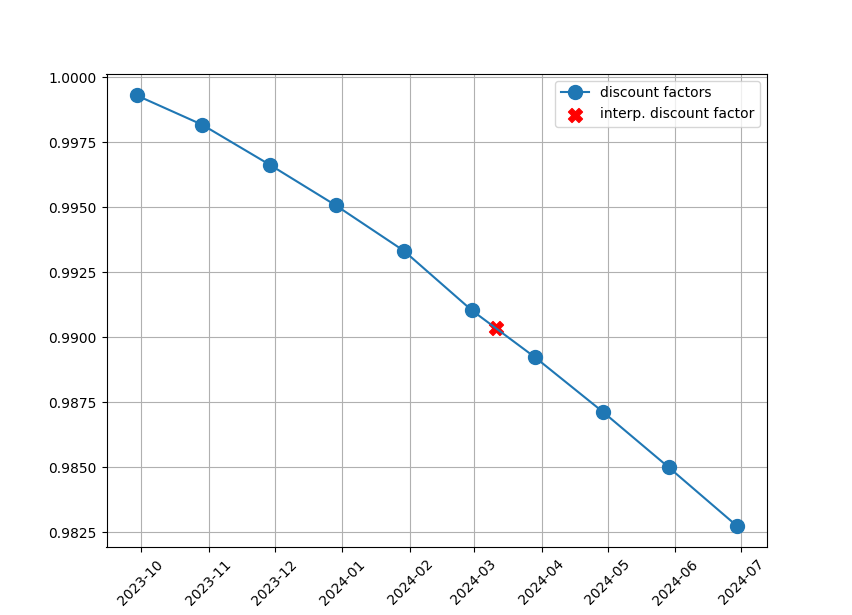
\includegraphics[width=1.\linewidth]{discount_interp}
        \end{center}
    \end{figure}
\end{columns}
\end{frame}



\begin{frame}{Forward Rates}
  \begin{itemize}
  \item A \emph{forward rate} is an interest rate applicable to a financial transaction that will take place in the future.
  \item It can be considered as the \emph{market expectation for future prices} and can serve as an indicator of how it believes will perform.
  \item Contrary the \emph{spot rate} is used by buyers and sellers looking to make an immediate purchase or sale.
  \item To calculate the forward rates exploit no-arbitrage argument:
    \begin{equation}
      \begin{gathered}
        e^{r_1 (t_1-t_0)}e^{r_{1,2}(t_2 - t_1)} = e^{r_2 (t_2-t_0)} \implies e^{r_1 t_1 + r_{1,2}(t_2 - t_1)} = e^{r_2 t_2} \\
        r_1 t_1 + r_{1,2}(t_2 - t_1) = r_2 t_2 \implies r_{1,2} = \cfrac{r_2 t_2 - r_1 t_1 }{t_2 - t_1}
      \end{gathered}
    \end{equation}
  \end{itemize}
\end{frame}

\begin{frame}{Forward Rate Class}
  \begin{itemize}
  \item Now let's implement a Forward Rate class. The \textbf{attributes} of this class are
      \begin{itemize}
      \item a set of pillar dates (corresponding to given spot rates), $t_0,...,t_{n}$;
      \item a set of spot rates, $r(t_0),...,r(t_{n})$.
      \end{itemize}
  \item The "behavior" of the object is to return a forward rate given a time interval (if necessary it must interpolate to get the missing spot rates).
  \end{itemize}
\end{frame}

\begin{frame}{Forward Rate Class}
  \begin{itemize}
  \item Now let's implement a Forward Rate class. The \textbf{attributes} of this class are
      \begin{itemize}
      \item a set of pillar dates (corresponding to given spot rates), $t_0,...,t_{n}$;
      \item a set of spot rates, $r(t_0),...,r(t_{n})$.
      \end{itemize}
  \item The "behavior" of the object is to return a forward rate given a time interval. We will split it into two methods
    \begin{itemize}
    \item a method to interpolate rate at a given date; 
    \item a method to compute the forward rate relative to a time period.
    \end{itemize}
  \end{itemize}
\end{frame}

\begin{frame}[fragile]{Forward Rate Class}
\begin{ipython}
from scipy.interpolate import interp1d

class ForwardRateCurve:
    def __init__(self, obs_date, pillars, rates):
        self.obs_date = obs_date
        self.pillar_days = [(p - obs_date).days/365 for p in pillars]
        self.interpolator = interp1d(self.pillar_days, rates)
    
    def interp_rate(self, d):
        d_frac = (d - self.obs_date).days/365
        if d < self.obs_date or d_frac > self.pillar_days[-1]:
            print (f"Cannot extrapolate rates (date: {d}).")
            return None, None
        else:
            return d_frac, self.interpolator(d_frac)
    ...
\end{ipython}
\end{frame}

\begin{frame}[fragile]{Forward Rate Class}
\begin{ipython}
    ...
    def forward_rate(self, d1, d2):
        d1_frac, r1 = self.interp_rate(d1)
        d2_frac, r2 = self.interp_rate(d2)
        if d1_frac is None or d2_frac is None:
            return None
        else:
            return (r2*d2_frac - r1*d1_frac)/(d2_frac - d1_frac)
\end{ipython}
\end{frame}

\begin{frame}[fragile]{Testing the Class}
\begin{ipython}
from datetime import date

obs_date = date(2020, 1, 1)
pillars = [date(2020, 1, 1),
           date(2021, 1, 1),
           date(2022, 7, 1)]
rates = [0.0221, 0.0241, 0.0243]

fc = ForwardRateCurve(obs_date, pillars, rates)
t1 = date(2021, 1, 1)
t2 = date(2022, 1, 1)
print (f"F({t1}, {t2}) = {fc.forward_rate(t1, t2):.4f}")
\end{ipython}
\begin{ioutput}
F(2021-01-01, 2022-01-01) = 0.0244
\end{ioutput}
\end{frame}

\end{document}
